% biography section
% 
% If you have an EPS/PDF photo (graphicx package needed) extra braces are
% needed around the contents of the optional argument to biography to prevent
% the LaTeX parser from getting confused when it sees the complicated
% \includegraphics command within an optional argument. (You could create
% your own custom macro containing the \includegraphics command to make things
% simpler here.)
%\begin{IEEEbiography}[{\includegraphics[width=1in,height=1.25in,clip,keepaspectratio]{mshell}}]{Michael
%Shell}
% or if you just want to reserve a space for a photo:

%\newpage
%\vspace{-30pt}
%\begin{biography}[{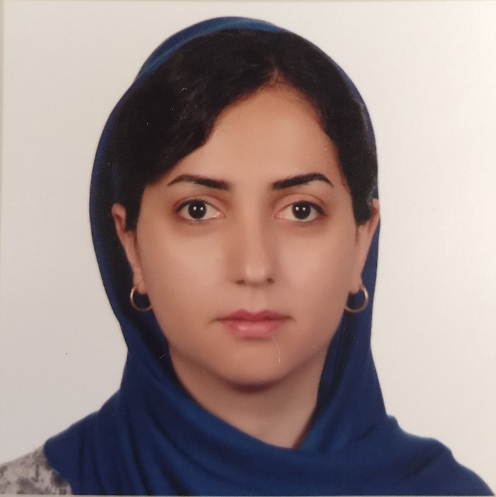
\includegraphics[height=1in,clip,keepaspectratio]{./figures/Zakieh.jpg}}]{Zakieh Sadat Hashemifar}
%is a 5th year Ph.D. student in Computer Science and Engineering at University at Buffalo. She has an undergraduate
%degree from Tehran University in 2010 and her masters
%degree from Sharif University of Technology in 2012, in Computer Science. Her research interests are in robotics, perception, SLAM and multi-robot applications. 
%\end{biography}
\section{Authors}
\begin{wrapfigure}{l}{25mm} 
    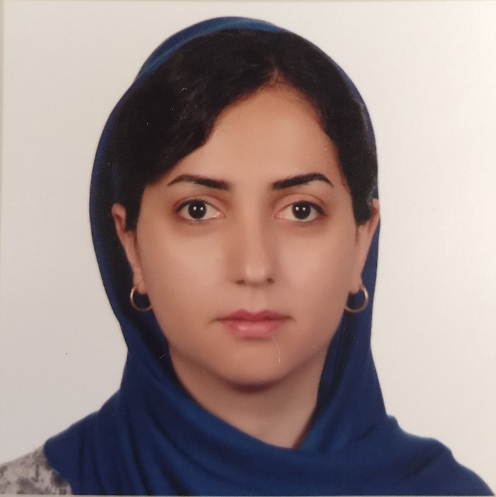
\includegraphics[width=1in,height=1in,clip,keepaspectratio]{./figures/Zakieh.jpg}
  \end{wrapfigure}\par
  \textbf{Zakieh S. Hashemifar} is a 5th year Ph.D. student in Computer Science and
Engineering at University at Buffalo. She has an undergraduate degree from
Tehran University in 2010 and her masters degree from Sharif University of
Technology in 2012, in Computer Science. Her research interests are in robotics,
perception, SLAM and multi-robot applications.\par
\begin{wrapfigure}{l}{25mm} 
    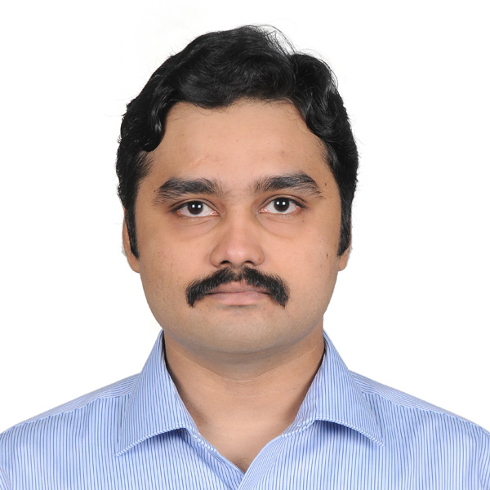
\includegraphics[width=1in,height=1in,clip,keepaspectratio]{./figures/Charu.jpg}
  \end{wrapfigure}\par
  \textbf{charuvahan Adhivarahan} is a 3rd year Ph.D. student in Computer Science and
Engineering at University at Buffalo. He received his Master's degree from the University at Buffalo and his Bachelor's degree from Annamalai University in India. His research interests are in robotics perception and multi-robot coordination.\par
\begin{wrapfigure}{l}{25mm} 
    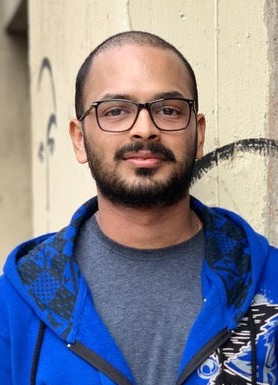
\includegraphics[width=1in,height=1in,clip,keepaspectratio]{./figures/Anand.jpg}
  \end{wrapfigure}\par
  \textbf{Anand Balakrishnan} is a 1st year Ph.D. student in the Department of Computer
Science at the University of Southern California. He completed his undergraduate degree in B.S. Computer Engineering at University at Buffalo, The State University of New York. His current research interests are in safety and validation in autonomous cyber-physical systems.\par
\begin{wrapfigure}{l}{25mm} 
    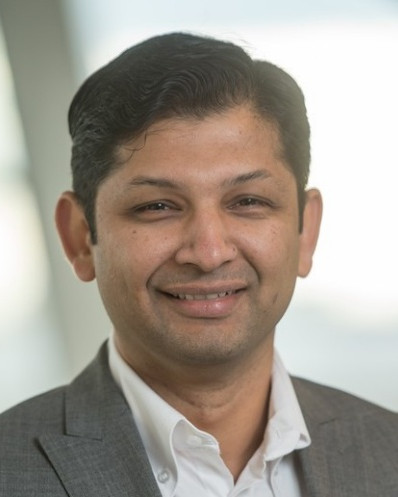
\includegraphics[width=1in,height=1in,clip,keepaspectratio]{./figures/Karthik.jpg}
  \end{wrapfigure}\par
  \textbf{Karthik Dantu} is currently an Assistant Professor in the Department of Computer
Science and Engineering at University at Buffalo, The State University of New
York. He received his Ph.D. from the University of Southern California in
Computer Science and his Bachelors degree from Mysore University in India. His
research interests are in sensing and coordination in mobile/robotic systems.\par

% if you will not have a photo at all:
%\vspace{-42pt}
%\begin{IEEEbiography}[{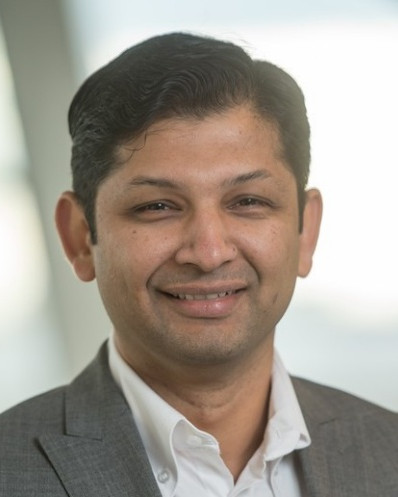
\includegraphics[height=1in,clip,keepaspectratio]{./figures/Karthik.jpg}}]{Karthik Dantu}
%is currently an Assistant Professor in the Department of Computer Science and Engineering at University at Buffalo, The State University
%of New York. He received his Ph.D. from the University of Southern California in Computer Science and his Bachelors degree from Mysore University in India. His research interests are in sensing and coordination in mobile/robotic systems.
%\end{IEEEbiography}


